\documentclass[12pt,letterpaper]{article}
\usepackage{graphicx,textcomp}
\usepackage{natbib}
\usepackage{setspace}
\usepackage{fullpage}
\usepackage{color}
\usepackage[reqno]{amsmath}
\usepackage{amsthm}
\usepackage{fancyvrb}
\usepackage{amssymb,enumerate}
\usepackage[all]{xy}
\usepackage{endnotes}
\usepackage{lscape}
\newtheorem{com}{Comment}
\usepackage{float}
\usepackage{hyperref}
\newtheorem{lem} {Lemma}
\newtheorem{prop}{Proposition}
\newtheorem{thm}{Theorem}
\newtheorem{defn}{Definition}
\newtheorem{cor}{Corollary}
\newtheorem{obs}{Observation}
\usepackage[compact]{titlesec}
\usepackage{dcolumn}
\usepackage{tikz}
\usetikzlibrary{arrows}
\usepackage{multirow}
\usepackage{xcolor}
\newcolumntype{.}{D{.}{.}{-1}}
\newcolumntype{d}[1]{D{.}{.}{#1}}
\definecolor{light-gray}{gray}{0.65}
\usepackage{url}
\usepackage{listings}
\usepackage{color}

\definecolor{codegreen}{rgb}{0,0.6,0}
\definecolor{codegray}{rgb}{0.5,0.5,0.5}
\definecolor{codepurple}{rgb}{0.58,0,0.82}
\definecolor{backcolour}{rgb}{0.95,0.95,0.92}

\lstdefinestyle{mystyle}{
	backgroundcolor=\color{backcolour},   
	commentstyle=\color{codegreen},
	keywordstyle=\color{magenta},
	numberstyle=\tiny\color{codegray},
	stringstyle=\color{codepurple},
	basicstyle=\footnotesize,
	breakatwhitespace=false,         
	breaklines=true,                 
	captionpos=b,                    
	keepspaces=true,                 
	numbers=left,                    
	numbersep=5pt,                  
	showspaces=false,                
	showstringspaces=false,
	showtabs=false,                  
	tabsize=2
}
\lstset{style=mystyle}
\newcommand{\Sref}[1]{Section~\ref{#1}}
\newtheorem{hyp}{Hypothesis}


\title{Problem Set 4}
\date{Due: December 4, 2022}
\author{Applied Stats/Quant Methods 1: 16327268, Marcus Ó Faoláin}


\begin{document}
	\maketitle
	\section*{Instructions}
	\begin{itemize}
		\item Please show your work! You may lose points by simply writing in the answer. If the problem requires you to execute commands in \texttt{R}, please include the code you used to get your answers. Please also include the \texttt{.R} file that contains your code. If you are not sure if work needs to be shown for a particular problem, please ask.
		\item Your homework should be submitted electronically on GitHub.
		\item This problem set is due before 23:59 on Sunday December 4, 2022. No late assignments will be accepted.
	\end{itemize}




	\vspace{.5cm}
\section*{Question 1: Economics}
\vspace{.25cm}
\noindent 	
In this question, use the \texttt{prestige} dataset in the \texttt{car} library. First, run the following commands:

\begin{verbatim}
install.packages(car)
library(car)
data(Prestige)
help(Prestige)
\end{verbatim} 


\noindent We would like to study whether individuals with higher levels of income have more prestigious jobs. Moreover, we would like to study whether professionals have more prestigious jobs than blue and white collar workers.

\newpage
\begin{enumerate}
	
	\item [(a)]
	Create a new variable \texttt{professional} by recoding the variable \texttt{type} so that professionals are coded as $1$, and blue and white collar workers are coded as $0$ (Hint: \texttt{ifelse}).
	\\\\
	\noindent We create a new variable \texttt{professional} in which professionals are coded as 1 and blue and white collar workers are coded as 0 using \texttt{ifelse}.
	\begin{lstlisting}
Prestige$professional <- ifelse(Prestige$type == "prof", 1, 0)
	\end{lstlisting}

\noindent We make sure the new variable has been added to the \texttt{Prestige} dataset by calling the \texttt{head()} function.
\begin{lstlisting}
head(Prestige)
\end{lstlisting}

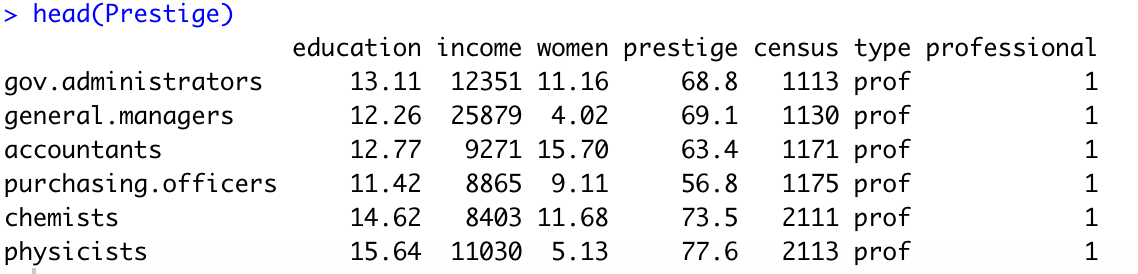
\includegraphics[width=\textwidth]{head(Prestige).png}	

\noindent Based on the output from the screenshot above, the code appears to have successfully added the new binary \texttt{professional} column.	
	
	\vspace{6cm}
	
\newpage	
	\item [(b)]
	Run a linear model with \texttt{prestige} as an outcome and \texttt{income}, \texttt{professional}, and the interaction of the two as predictors (Note: this is a continuous $\times$ dummy interaction.)
\\\\
\noindent We run a linear model with \texttt{prestige} as an outcome and \texttt{income}, \texttt{professional} and the interaction of the two as predictor variables. \texttt{Professional}, with it's binary values of 0 and 1, acts as a dummy variable in this case. We format the model using a * multiplication symbol instead of an + addition symbol to show that it is an interactive rather than additive model.

\begin{lstlisting} 
prestige.lm <- lm(prestige ~ income * professional, data = Prestige)
\end{lstlisting}

\noindent Running a summary call on the model yields output in the console, which is shown through the following image file	
	
\begin{lstlisting} 
summary(prestige.lm)
\end{lstlisting}

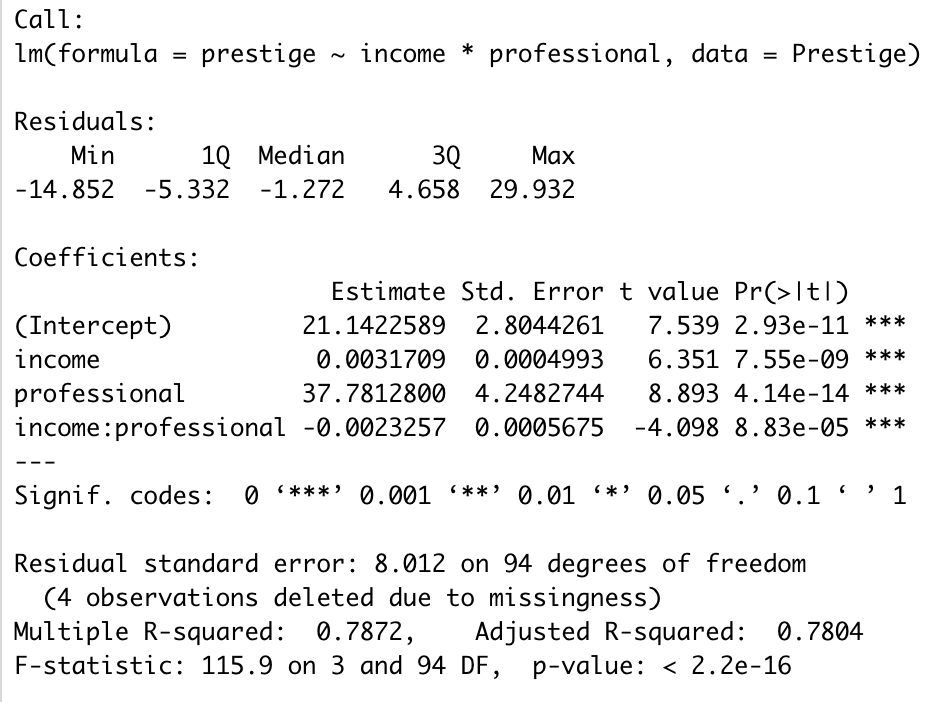
\includegraphics[width=\textwidth]{Prestige.lm.png}
	
	\vspace{6cm}
	\item [(c)]
	Write the prediction equation based on the result.
	
\noindent The formula for the prediction eqaution for a model with an interaction term is as follows:

\[Y_i = \beta_o + \beta_1X_i + \beta_2D_i + \beta_3X_iD_i + \varepsilon_i\]

\noindent In our case, $Y_i$is prestige, $\beta_o$ is the intercept, $\beta_1$ is the beta coefficient of \texttt{income}, $X_i$ is the \texttt{income} variable, $\beta_2$ is the beta coefficient of the \texttt{professional} variable, $D_i$ is whether someone is \texttt{professional} or not, $\beta_3$ is the coefficient of the interaction between the terms and $\epsilon_i$ is the error term.
\\\\
\noindent From our results, the intercept $\beta_0$ has a value of 21.1422589, our coefficient of \texttt{income} $\beta_1$ has a value of 0.0031709, our \texttt{professional} coefficient $\beta_2$ has a value of 37.7812800 and the coefficient of our interaction between \texttt{income} and \texttt{professional} $\beta_3$ is -0.0023257.
\\\\
\noindent Therefore, our generalised linear equation for \texttt{prestige} is as follows:
\\
\[Y_i = 21.142 + 0.0031709X_i + 37.781D_i -0.0023257X_iD_i\]
\\
\noindent For professionals, $D_i$ takes a value of 1, therefore for professionals the linear equation for \texttt{prestige} is as follows:
\\
\[Y_i = 21.142 + 0.0031709X_i + 37.781 - 0.0023257X_i\]
\\
\noindent Simplified, the linear equation for \texttt{prestige} for professionals is:
\\
\[Y_i = 58.923 + 0.0008452X_i\]
\\
\noindent In the linear equation for non-professionals, $D_i$ takes a value of 0, so the linear equation for \texttt{prestige} for non professionals is as follows:
\\
\[Y_i = 21.142 + 0.0031709X_i\]
	
\newpage
	\item [(d)]
	Interpret the coefficient for \texttt{income}.
\\\\
\noindent The coefficient for income is the amount by which our outcome variable, \texttt{prestige} will increase by, if our income is increased by one unit, if all other variables are kept constant.
\\\\
\noindent In practice, this means an increase in \texttt{income} of 1 will result in a 0.0031709 increase in \texttt{prestige}, if all other variables are kept constant.

	\vspace{5cm}	
	\item [(e)]
	Interpret the coefficient for \texttt{professional}.
\\\\
\noindent The coefficient for \texttt{professional} is the amount by which \texttt{prestige} changes on average depending on whether one is professional or non-professional, keeping all other variables constant.
\\\\
\noindent In practice this means that, keeping all other variables constant, being a professional results in a 37.781 increase in \texttt{prestige} on average versus not being a professional.
	
	\newpage
	\item [(f)]
	What is the effect of a \$1,000 increase in income on prestige score for professional occupations? In other words, we are interested in the marginal effect of income when the variable \texttt{professional} takes the value of $1$. Calculate the change in $\hat{y}$ associated with a \$1,000 increase in income based on your answer for (c).
\\\\
\noindent To answer this question, we must use the first formula for \texttt{prestige} for professionals from part (c), namely:
\[Y_i = 58.923 + 0.0008452X_i\]
\\
\noindent To calculate the marginal effect on \texttt{prestige} of a \$1000 increase in income for professionals, we can calculate the value of \texttt{prestige} at two different income values \$1000 apart.
\\\\
\noindent We shall take these \texttt{prestige} values at \$0 and at \$1000.
\\\\
\noindent At \$0
\[Y_1 = 58.923 + 0.0008453(0)\]
\[Y_1 = 58.923\]
\\\\
\noindent At \$1000
\[Y_2 = 58.923 + 0.0008452(1000)\]
\[Y_2 = 58.923 + 0.8452\]
\[Y_2 = 59.7682\]
\\
\noindent To calculate the change in $\hat{y}$, we subtract $Y_1$ from $Y_2$.
\\
\[Y_2 - Y_1\]
\[= 59.7682 - 58.923\] 
\[= 0.8452\]
\\
\noindent Therefore, the marginal effect of income on \texttt{prestige} on for professionals is 0.8452. This means a \$1000 increase in income for professionals results in a 0.8452 increase in \texttt{prestige}.
	\vspace{10cm}
	
	
	\item [(g)]
	What is the effect of changing one's occupations from non-professional to professional when her income is \$6,000? We are interested in the marginal effect of professional jobs when the variable \texttt{income} takes the value of $6,000$. Calculate the change in $\hat{y}$ based on your answer for (c).
\\\\
\noindent We can calculate the effect of changing one's occupation from non-professional to professional when income is \$6,000 using the two formulae for professional and non-professional discovered in (c).
\\\\
\noindent For professionals:
\[Y_i = 58.923 + 0.0008452X_i\]
\\
\noindent For non-professionals:
\[Y_i = 21.142 + 0.0031709X_i\]
\\
\noindent We set the value of $X_i$ to \$6,000 for each linear equations.
\\\\
\noindent For professionals:

\[Y_p = 58.923 + 0.0008452(6,000)\]
\[Y_p = 58.923 + 5.0712\]
\[Y_p =63.9942\]
\\\\
\noindent For non-professionals:

\[Y_n = 21.142 + 0.0031709(6,000)\]
\[Y_n = 21.142 + 19.0254\]
\[Y_n = 40.1674\]	
\\
\noindent To calculate the effect of changing one's occupation from non-professional to professional when income is \$6,000 ($\Delta Y$), we subtract $Y_n$ from $Y_p$.
\\
\[\Delta Y = Y_p - Y_n\]
\[\Delta Y =(63.9942) - (40.1674)\]
\[\Delta Y = 23.8268\]
\\
\noindent This means that a change from a non-professional role to a professional role results in a 23.8268 increase in the outcome variable \texttt{prestige}.
	
\end{enumerate}

\newpage

\section*{Question 2: Political Science}
\vspace{.25cm}
\noindent 	Researchers are interested in learning the effect of all of those yard signs on voting preferences.\footnote{Donald P. Green, Jonathan	S. Krasno, Alexander Coppock, Benjamin D. Farrer,	Brandon Lenoir, Joshua N. Zingher. 2016. ``The effects of lawn signs on vote outcomes: Results from four randomized field experiments.'' Electoral Studies 41: 143-150. } Working with a campaign in Fairfax County, Virginia, 131 precincts were randomly divided into a treatment and control group. In 30 precincts, signs were posted around the precinct that read, ``For Sale: Terry McAuliffe. Don't Sellout Virgina on November 5.'' \\

Below is the result of a regression with two variables and a constant.  The dependent variable is the proportion of the vote that went to McAuliff's opponent Ken Cuccinelli. The first variable indicates whether a precinct was randomly assigned to have the sign against McAuliffe posted. The second variable indicates
a precinct that was adjacent to a precinct in the treatment group (since people in those precincts might be exposed to the signs).  \\

\vspace{.5cm}
\begin{table}[!htbp]
	\centering 
	\textbf{Impact of lawn signs on vote share}\\
	\begin{tabular}{@{\extracolsep{5pt}}lccc} 
		\\[-1.8ex] 
		\hline \\[-1.8ex]
		Precinct assigned lawn signs  (n=30)  & 0.042\\
		& (0.016) \\
		Precinct adjacent to lawn signs (n=76) & 0.042 \\
		&  (0.013) \\
		Constant  & 0.302\\
		& (0.011)
		\\
		\hline \\
	\end{tabular}\\
	\footnotesize{\textit{Notes:} $R^2$=0.094, N=131}
\end{table}

\vspace{.5cm}
\begin{enumerate}
\newpage
	\item [(a)] Use the results from a linear regression to determine whether having these yard signs in a precinct affects vote share (e.g., conduct a hypothesis test with $\alpha = .05$).
\\\\	
\noindent We can use the results of the linear regression above to create a linear equation for the impact of lawn signs on vote share. The formula for linear relationships is as follows:
\\\\
\[Y = \beta_0 + \beta_1X_1 + \beta_2X_2 + \varepsilon \]	

\noindent where y is the proportion of vote that went to Cucinelli, $\beta_0$ is the constant term, $\beta_1$ is the coefficient of the variable for a precinct having a lawn sign assigned, $X_1$ is the variable for whether the precint has the lawn sign assigned, $\beta_2$ is the coefficient of the variable for whether the precinct is adjacent to a precint with a lawn sign, $X_2$ is the variable for whether a precinct has a sign adjacent to it and $\varepsilon$ is the error term.
\\\\
\noindent By putting in the results from the table, we can get the following equation:
\\\\
\[Y = 0.302 + (0.042)X_1 + (0.042)X_2\]
\\\\
\noindent The question above asks us to determine whether having these yard signs in a precinct affects vote share. This means we have to see whether having a yard sign in one's 
precinct has an effect on vote share. To see if it has an effect, we must investigate whether $\beta_1$ (0.042), the coefficient for $X_1$, is equal to zero or not
\\\\
\noindent Our null hypothesis, $H_0$, states that the coefficient of the variable for precincts assigned with lawn signs, $\beta_1$, is equal to 0.
\\\\
\noindent Our alternative hypothesis, $H_\alpha$, states that the coefficient of the variable for precincts assigned with lawn signs, $\beta_1$, is not equal to 0.
\\\\
\[H_0:\beta_1 = 0\]
\[H_\alpha: \beta_1  \neq  0\]
\\\\
\noindent In order to perform a hypothesis test, we must calculate a t-statistic for beta 1. We do this using the formula:
\\\\
\[ t= \frac{\hat{\beta_0} - \beta_0}{se} \]
\\\\
\noindent Substituting in the values and calculating values through code in R, we get:
\\\\
\begin{lstlisting}
t.statistic.assigned <- (assigned.b1) / (assigned.se)
t.statistic.assigned
\end{lstlisting}
\[ t= \frac{0.042 -0}{0.016} \]
\[t = 2.65\]
\\\\
\noindent We must also calculate the critical values of a two tailed t distribution at a significance level of $\alpha = 0.05$ .
\\\\
\noindent If the value of our "assigned" t-statistic is greater than the critical value of the t-distribution, we can reject the null hypothesis and conclude that $\beta_1 \neq 0$.
\\\\
\noindent This would mean that a precinct having these yard signs does affect vote share.
\\\\
\noindent We can calculate the critical value with the \texttt{qt()} function in R.
\\\\
\noindent We use a p-value of 0.05/2 since it is a two tailed t-test, one used simply measure if there is an effect rather than how much that effect is. 
\\\\
\noindent We get our degrees of freedom using the formula $df = n-3$, where n is the total number of observations and 3 is the number of estimated coefficients.

\begin{lstlisting}
df.b1 <- 131 - 3
qt(p = 0.05/2, df = df.b1, lower.tail = FALSE)
\end{lstlisting}

\noindent This gives us a critical value of 1.978671.
\\\\
\noindent Since this critical value of 1.978671 is less than the t-statistic of 2.65, we can reject the null hypothesis that having yard signs in a precinct has no effect on voteshare. This means that $\beta_1$ is not equal to zero. ($\beta_1 \neq 0$)
\\\\
\noindent We can therefore conclude that having these yard signs in a precinct does in fact affect vote share. 


	\newpage		
	\item [(b)]  Use the results to determine whether being
	next to precincts with these yard signs affects vote
	share (e.g., conduct a hypothesis test with $\alpha = .05$).
\\\\	
\noindent Part (b) asks us to perform a hypothesis test on the second coefficient in the equation, $\beta_2$. This is the coefficient for the variable for precincts adjacent to lawn signs, $X_2$. We can perform a  similar hypothesis test to the one in part (a).
\\\\
\noindent To see if having a lawn sign in an adjacent precinct has an effect on voteshare or not, we must investigate whether $\beta_2$, the coefficient for $X_1$ is equal to zero or not.
\\\\
\noindent Our null hypothesis, $H_0$, states that the coefficient of the variable for precincts adjacent to those with lawn signs, is equal to zero.
\\\\
\noindent Our alternative hypothesis, $H_\alpha$, states that the coefficient of the variable for precincts adjacent to those with lawn signs is not equal to zero.
\\\\
\[H_0: \beta_2 = 0\]
\[H_\alpha: \beta_2 \neq 0\]
\\\\
In order to perform a hypothesis test for $\beta_2$, we must calculate a t-statistic. We do this using the following formula:
\\\\
\[ t= \frac{\hat{\beta_0} - \beta_0}{se} \]
\\\\
\noindent Substituting in values and calculating it in R, we get the following:
\begin{lstlisting}
t.statistic.adjacent <- (adjacent.b2) / (adjacent.se)
t.statistic.adjacent
\end{lstlisting}
\[ t= \frac{0.042 - 0}{0.013} \]
\[ t= 3.230769\]
\\\\
\noindent We must also calculate the critical values of a two tailed t distribution at a significance level of $\alpha = 0.05$.
\\\\
\noindent If the value of our "adjacent" t-statistic is greater than the the critical value of the t-distribution, we can reject the null hypothesis and conclude that $\beta_2 \neq 0$.
\\\\
\noindent This would mean that being adjacent to a precinct with the anti-McAuliffe yard signs does affect voter share. 
\\\\
\noindent We can calculate the critical value with the \texttt{qt()} function in R.
\\\\
\noindent We use a p=value of 0.05/ 2 since it is a two tailed t-test.
\\\\
\noindent We get out degrees of freedom using the formula df = n-3, where n is the total number of observations and 3 is the number of estimated coefficients.
\begin{lstlisting}
df.b2 = 131-3
qt(p = 0.05/2, df = df.b2, lower.tail = FALSE)
\end{lstlisting}
\noindent The critical value is 1.978671, the same as in the part (a).
\\\\
\noindent Since the critical value of 1.978671 is less than the t-statistic of 3.230769, we can reject the null hypothesis that having yard signs in a precinct has no effect on vote share. This means that $\beta_2$ is not equal 0. ($\beta_2 \neq 0$).
\\\\
\noindent We can therefore conclude that these yard signs being present in an adjacent precinct does in fact affect vote share.

\newpage
	\vspace{7cm}
	\item [(c)] Interpret the coefficient for the constant term substantively.
\\\\
\noindent The coefficient $\beta_0$ for the constant term is the point at which the regression line crosses the y-axis. This means it is the value of y when $X_1$ is equal to zero and $X_2$ is equal to zero.
\\\\
\noindent What this means in practice is that it is the proportion of vote share that is predicted to go to Cuccinelli in precincts that neither have the anti-McAuliffe yard signs nor are adjacent to precincts with the anti-McAuliffe yard signs.
\\\\
\noindent This means that we would expect Cuccinelli to receive around 30.2\% of the vote share in precincts that neither have the lawn signs nor are adjacent to those with the lawn signs.

	
\newpage	
	\item [(d)] Evaluate the model fit for this regression.  What does this	tell us about the importance of yard signs versus other factors that are not modeled?
\\\\
\noindent The $R^2$ value of 0.094 tells us the proportion of total variance accounted for by the regression model. This means that around 9.4\% of the variance of the model is accounted for by the model, which means around 90.6\% of the variance of the outcome variable is not accounted for by it. 
\\\\
\noindent This means that a very large proportion, over 90\%, of the variance of the outcome variable is not accounted for by the model. This suggests to us that other factors combined are far more important in explaining the variance of the outcome variable than the yard signs.
\\\\
\noindent While the yard signs do have some effect on that variance of the vote share, it would be important to consider it as only one small part of all the factors that affected vote share in this election.
	
\end{enumerate}  


\end{document}